
\subsection{Using the Frobenius eigenvalue of $P(s)$}

\noindent
An expression which seems to be succesful for the variance is :

\centers{$  \left( \ddot{\lambda}(-1) - { \dot{\lambda}(-1) }^2 \right) \f{n}{\ln^2 n} $}

\noindent Let's compute $\ddot{\lambda}(-1)$ with a Markov chain of order 1.

\leftcenters
    {In the paper,}
    {$ \ddot{\lambda}(-1) = \pi \ddot{P}(-1)\psi
                        + 2 \dot{\pi}(-1) \dot{P}(-1) \psi
                        - 2 \dot{\lambda}(-1) \dot{\pi}(-1) \psi $}
\noindent However, the relations defining $\pi(s)$ : 
   
        \centers{ $ \left\{
            \begin{array}{rl} \pi(s) P(s)  &= \lambda(s) \pi(s) \\
                          P(s) \psi(s) &= \lambda(s) \psi(s) \\
                          \pi(s) \psi(s) &= \lambda(s) 
            \end{array}
                    \right. $}
         
did not seem to allow me to directly compute $\dot{\pi}(s)$ (it seemed like I need
one more).
Therefore, I computed $\lambda(s)$ as the greatest 
eigenvalue of $P(s)$. Let $\chi$ the characteristic polynomial of $P(s)$,
and $\Delta$ its discrimant

\centers{$ \chi = (X - {p_{0 0}}^{-s}) 
                  (X - {p_{1 1}}^{-s}) 
                    - (p_{0 1} \, p_{1 0})^{-s} $}

\begin{egalites}
 and   & \Delta 
        & (\poo + \pii)^2 - 4[\pooii - \poiio] \\[2mm]
        && {p_{0 0}}^{-2s} 
                + {p_{1 1}}^{-s} - 2\pooii + 4\poiio
\end{egalites}

 Informally, we have this expression for $\lambda(s)$ 
where we need to decide which sign is the correct one :
\encadre{$ \lambda(s) = \f{ \poo + \pii \pm \sqrt{\Delta(s)}}{2} $}

\leftcenters
    {Since}
    {$\Delta(-1) 
        = (p_{0 0} + p_{1 1})^2 
                        - 2 p_{0 0} p_{1 1} 
                        + 4 p_{0 1} p_{1 0}
        = (p_{0 0} + p_{1 1} - 2)^2 $}
then $ \sqrt{ \Delta(-1) } = 2 - p_{0 0} - p_{1 1} = p_{0 1} + p_{1 0}$. 
Thus, picking the $+$ sign in the former expression, we verify that  
\centers{$ \lambda(-1) =  \f{ p_{0 0} + p_{1 1} + \sqrt{ \Delta(-1) } }
                                               {2} = 1 $}

\leftcenters
    {Derivating}
    {$ \dot{\lambda}(s) = \f12 \left( -\ln p_{0 0}\, \poo - \ln p_{1 1}\, \pii + \f{ \Delta'(s) }{ 2 \sqrt{\Delta(s)} } \right) $}

and the expression for $\Delta'(s)$
\centers{$ \Delta'(s) = - 2 \ln p_{0 0}\, \poodeux - 2 \ln p_{1 1}\, \piideux
                        + 2 \ln (p_{0 0} p_{1 1})\, \pooii 
                        - 4 \ln (p_{0 1} p_{1 0})\, \poiio $}
gives
\centers{$ \Delta'(-1) = - 2 \ln p_{0 0}\, {p_{0 0}}^2 - 2 \ln p_{1 1}\, {p_{1 1}}^2
                        + 2 \ln (p_{0 0} p_{1 1})\, (p_{0 0} p_{1 1})
                        - 4 \ln (p_{0 1} p_{1 0})\, (p_{0 1} p_{1 0})  $}

allowing to compute $\dot{\lambda}(-1)$. 
Numerically, we verified that $ \dot{\lambda}(-1) = h $. Derivating again yields

\centers{$ \ddot{\lambda}(s) =
                \f12 \left( \ln^2 p_{0 0} \poo + \ln^2 p_{1 1} \pii
                    + \f{ \Delta''(s) \sqrt{\Delta(s)} - \Delta'(s) \cdot \tf{\Delta'(s)}
                                                                            {2\sqrt{\Delta(s)}} }
                        {2\Delta(s)} \right)
                   $}

\leftcenters
    {with}
    {$ \Delta''(s) = 4 \ln^2 p_{0 0}\, \poodeux + 4 \ln^2 p_{1 1}\, \piideux
                     - 2 \ln^2 (p_{0 0} p_{1 1})\, \pooii
                     + 4 \ln^2 (p_{0 1} p_{1 0})\, \poiio $}

\leftencadre
    {Finally}
    {$\ddot{\lambda}(-1) = \f12 \left( \ln^2 p_{0 0}\, p_{0 0} + \ln^2 p_{1 1}\, p_{1 1}
                                + \f{ \Delta''(-1) \sqrt{\Delta(-1)} - \tf { {\Delta'(-1)}^2 }
                                                                              {2\sqrt{\Delta(-1)}} }
                                        {2\Delta(-1)} \right)
                         $}

The simulations using this coefficient for the variance are quite good. It also seems that 
this formula for the variance is equivalent to the one used in the unpublished paper 
\emph{Probabilistic Analysis of Lempel-Ziv Parsing for Markov Sources} by Leckey, 
Wormald and Neininger, but our two ways of deriving it differs. Numerical instability
might account for the tiny differences found for high $n$ values ($10^7$), although
this hasn't been verified. 
The code that computes it can be found in appendix \ref{app:comp_lam2}, and another 
way of computing $\lambda(s)$ is in appendix \ref{app:comp_lam1}.

\centers{
 	 \begin{minipage}{11cm}
        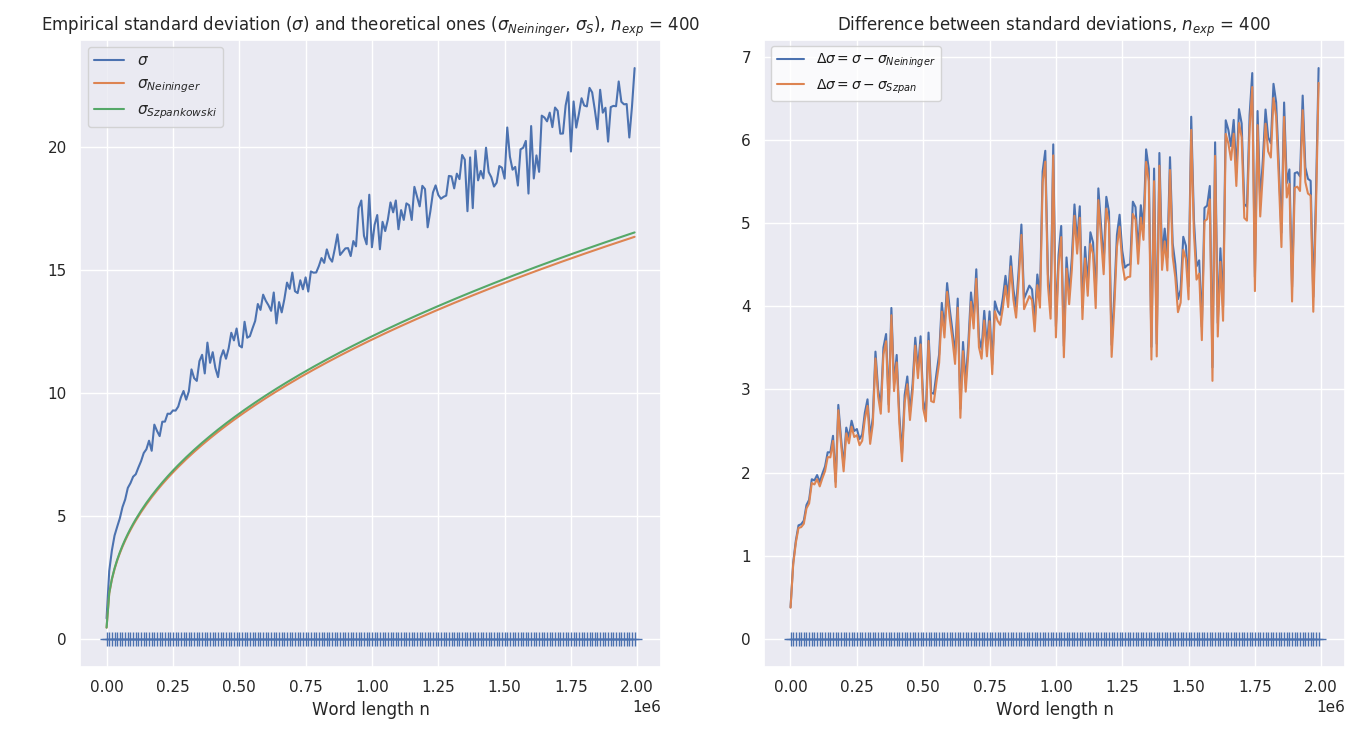
\includegraphics[width = 11cm,
        				    trim = 0 0 16.5cm 0,
        				    	clip=true]{./figs/eig_fig1.png}	
	\end{minipage} 
	}

\centers{
 	 \begin{minipage}{11cm}
        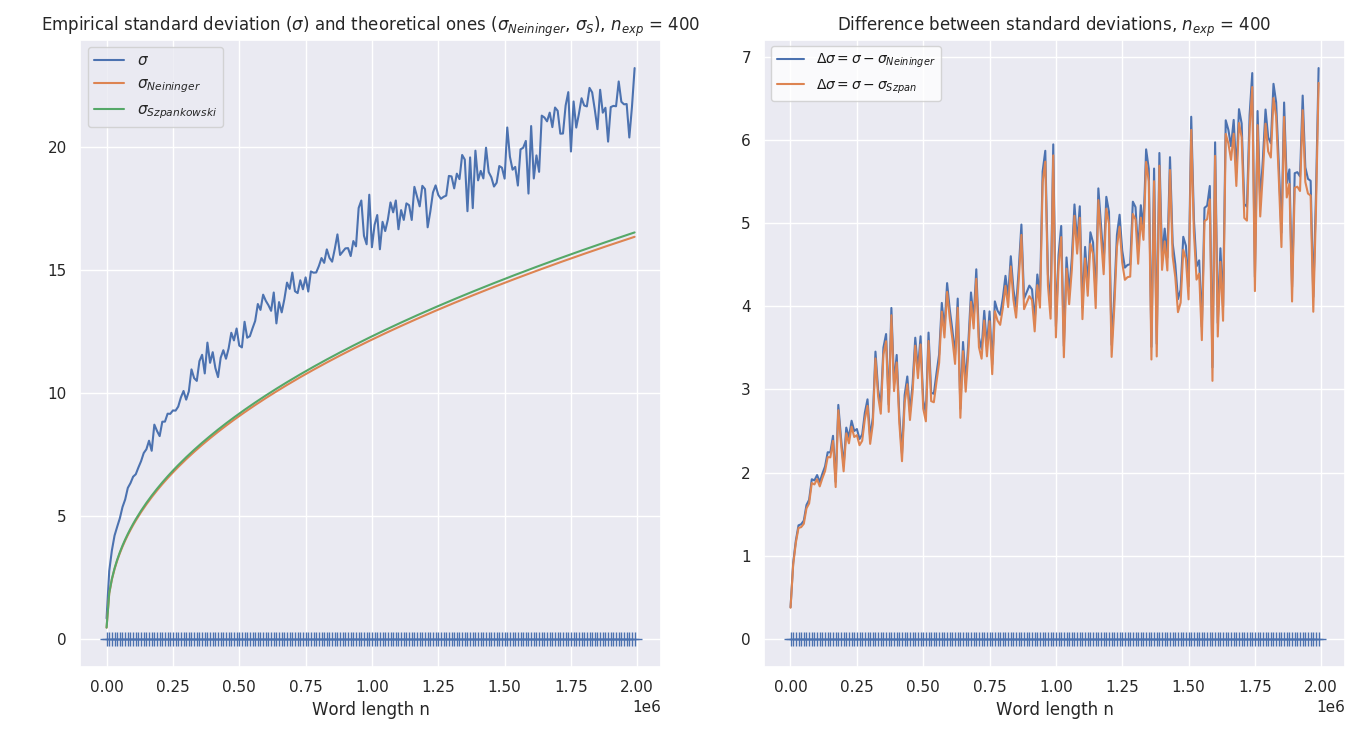
\includegraphics[width = 11cm,
        				    trim = 18.5cm 0 0 0,
        				    	clip=true]{./figs/eig_fig1.png}	
	\end{minipage} 
	}

\pagebreak
Now, for some distributions of very long words that were normalized using 
our theoretical standard deviations, and empirical means. The blue plot is 
a gaussian fit for the simulation results, which also appear as a blue histogram.
The two sets of figures are identical but obtained using different expressions.

\noindent
 	 \begin{minipage}{\textwidth}
        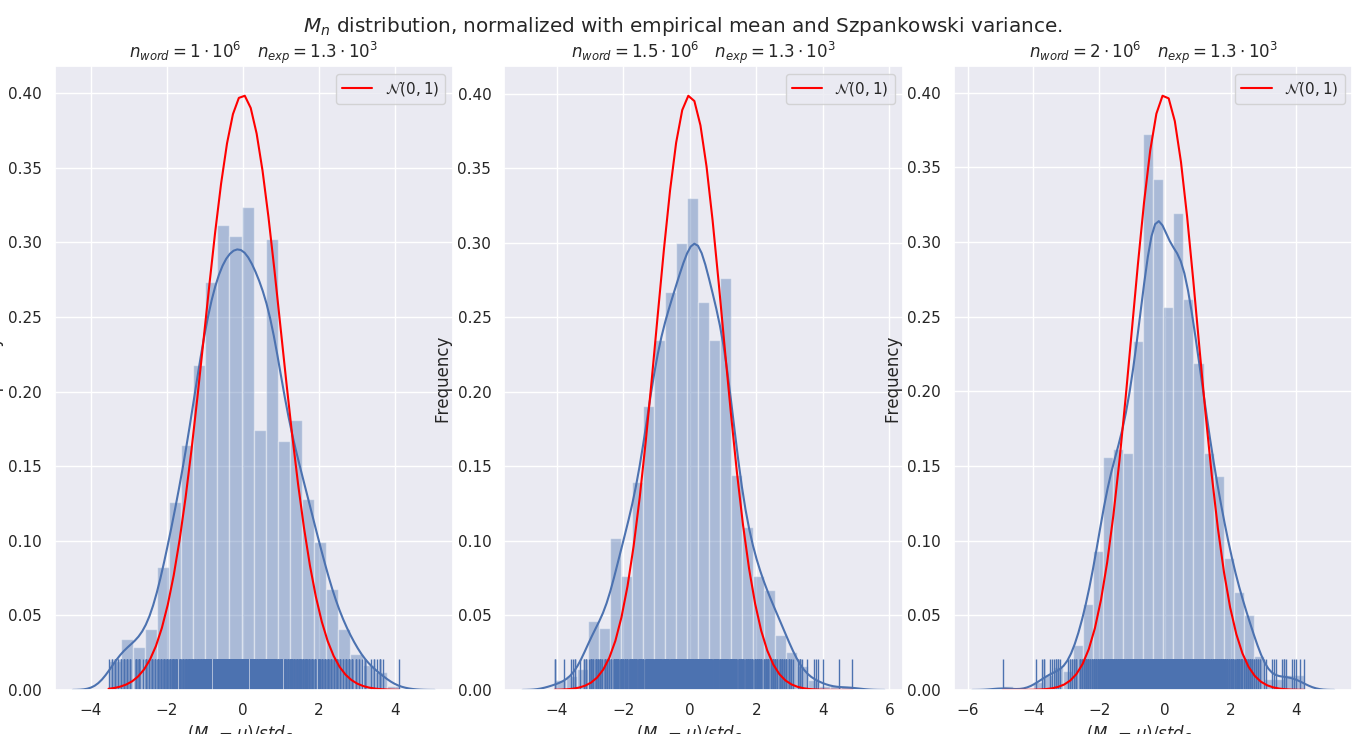
\includegraphics[width = \textwidth,
        				    trim = 0 0.5cm 0 0,
        				    	clip=true]{./figs/eig_fig2.png}	
	\end{minipage} 

\noindent
 	 \begin{minipage}{\textwidth}
        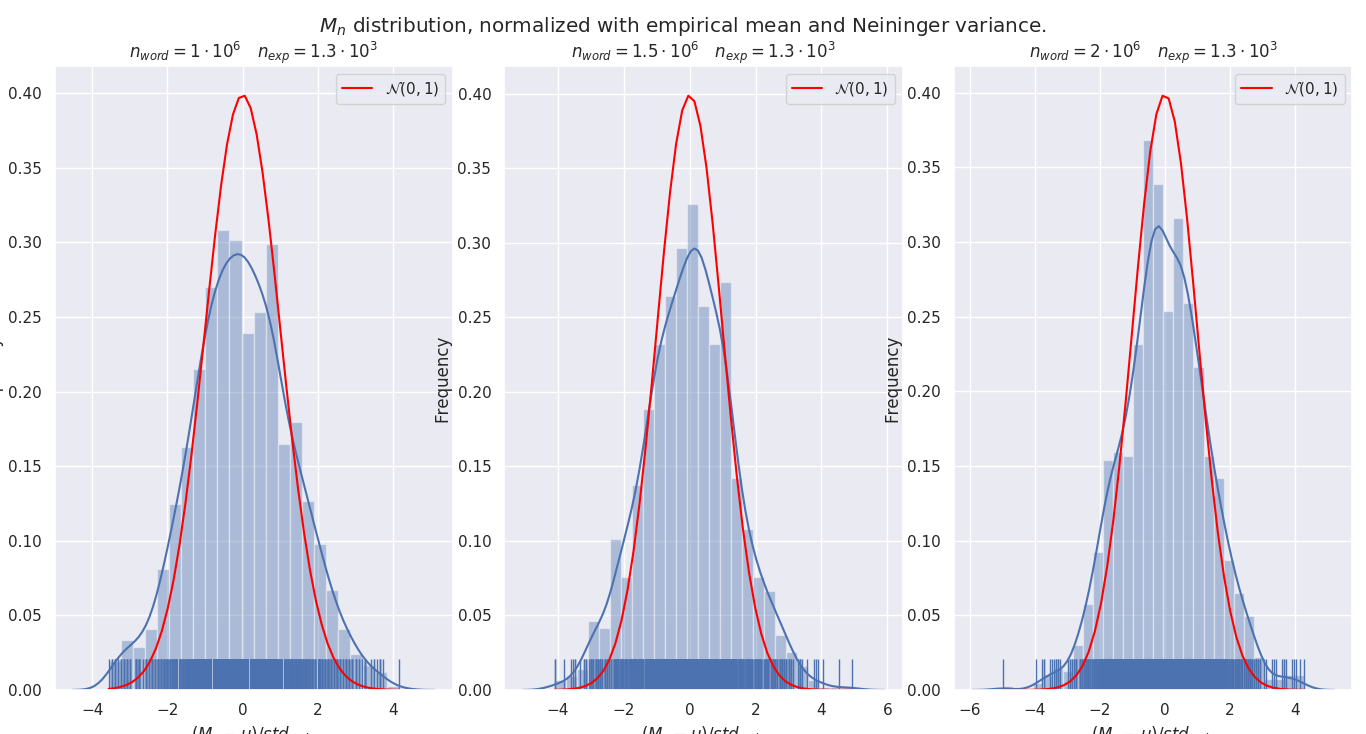
\includegraphics[width = \textwidth,
        				    trim = 0 0.5cm 0 0,
        				    	clip=true]{./figs/eig_fig3.png}	
	\end{minipage} 


\section{Conclusion}
Similar results were obtained for a variety of randomly generated Markov sources,
which seem to indicate that this formula for the variance could be proven theoretically
correct. 

\begin{remarque}
\noindent \textbf{Limits of this work}


The figures suffer from imprecision over the computation of the empirical 
variance : this is due to the difficulties encountered in computing large amounts
of long words (of size over $10^6$). Possible ideas of improvement might come from parallelization,
rewriting functions in a computationnal language such as Julia, or using/devising a datastructure
specific to the task of building very long words.

Another problem is that the space of random Markov chains (here: stochastic matrices
of size 2) is not sampled thoroughly, therefore this claim might only seem to hold for some
specific Markov chains. Sampling a small number of Markov chains uniformly
according to their entropy might be interesting as a representation of the space,
 because otherwise it would be hard to sample a large number of stochastic matrices
due to the necessity of computing large words for each of them.

\end{remarque}


\begin{appendices}
\section{First lambda computation}
\label{app:comp_lam2}
\lstinputlisting[firstline=156,lastline=206]{../src/eigenvalues.py}



\section{Another (more complicated) computation of $\ddot{\lambda}(-1)$}
\label{app:comp_lam1}
This expression gives the sames numerical results as the first one, 
but is more complex to compute for no apparent gain other than having 
yet another similar way of computing $\ddot{\lambda}(-1)$. 
Computing $\delta(s)$, a complex root of 
$\Delta(s)$, writing $\Delta$ as :

\begin{calculs}
    & \Delta 
        &=& \underbrace{p_{0 0}^{-2\Re(s)} \cos(2\ln(p_{0 0})\Im(s))}_{a_0(s)} \\[6mm]
          &&+& \underbrace{p_{1 1}^{-2\Re(s)} \cos(2\ln(p_{1 1})\Im(s))}_{a_1(s)} \\[6mm]
           &&& \underbrace{- 2 (p_{0 0}\,p_{1 1})^{-\Re(s)} \cos(\ln(p_{0 0}\,p_{1 1})\Im(s))}_{a_2(s)} \\[6mm]
           &&+&  \underbrace{4 (p_{0 1}\,p_{1 0})^{-\Re(s)} \cos(\ln(p_{0 1}\,p_{1 0})\Im(s))}_{a_3(s)} \\[6mm]
          &&+& i \Im(\Delta) 
\end{calculs}

where $\Im(\Delta) = b_0(s) + b_1(s) + b_2(s) + b_3(s)$, with each $b_i(s)$ being
the same term as $a_i(s)$ with $\cos$ replaced by $\sin$. Writing

\centers{$\Delta = \alpha(s) + i \beta(s)$}

and searching for $\delta = x(s) + i y(s)$, meaning that

\centers{$ \left\{
                \begin{array}{rl}
                    x^2 - y^2 &= \alpha \\
                    2\, x\, y &= \beta \\
                    x^2 + y^2 &= \sqrt{\alpha^2+\beta^2}
                \end{array}
            \right.
        $}
    

This yields
 
    \centers{$
        \left\{
            \begin{array}{rl}
                     x &= \pm \sqrt{\f{1}{2}(\sqrt{\alpha^2+\beta^2}+\alpha)} \\
                     y &= \pm \sqrt{\f{1}{2}(\sqrt{\alpha^2+\beta^2}-\alpha)} 
            \end{array}
        \right. 
            $}

and since $2xy = \beta$, there is $\epsilon \in \{-1,1\}$ such that
             \centers{$ \delta = \pm (x + \ir \epsilon y) $}

\leftcenters    
    {so}
    {$\lambda(s) = \f{ \poo + \pii \pm (x + \ir \epsilon y)}{2}$}

\leftcenters
    {\text{i.e.}}
    {$\ddot{{\lambda}}(-1) = \f{ p_{0 0} \ln^2(p_{0 0})
                                    + p_{1 1} \ln^2(p_{1 1})
                                    \pm (\ddot{{x}}(-1) + \ir \epsilon \ddot{{y}}(-1))}
                                  {2} $}
where we'll have to find what is $\epsilon$ and which sign to pick.

But first, computing the derivatives of $x(s) = \sqrt{f(s)} $:
    \centers{$\dot{x}(s) = \f{f'(s)}{2x(s)}$}
    \leftcenters
        {and}
        {$\ddot{{x}}(s) = \f{ f''(s) x(s) - f'(s) \cdot \f{f'(s)}{2x(s)} }
                                   { 2 x^2(s) } $}

and then computing $f(s)$ :

    \centers{$ f(s) = \f12 (\sqrt{\alpha^2+\beta^2} + \alpha) $}
    \centers{$ f'(s) = \f12 \left[ \f{ \overbrace{ \dot{\alpha}\alpha + \dot{\beta}\beta }^{ \gamma(s) } }
                                     { \underbrace{\sqrt{\alpha^2 + \beta^2}}_{\kappa(s)} }
                                    + \dot{\alpha} \right] $}

    \leftcenters{with}{$ \dot{\alpha} = \dot{a_0} + \dot{a_1} + \dot{a_2} + \dot{a_3} $}

\leftcenters
    {As for $f''(s)$, it is}
    {$ f''(s) = \f12 \left[ 
                        \f{ \dot{\gamma}(s) \kappa(s) - \gamma(s) \dot{\kappa}(s) }
                          {\kappa^2(s)} 
                        + \ddot{{\alpha}}(s) 
                    \right] $}

\leftcenters
    {with}
    {$\dot{\gamma}(s) = \ddot{{\alpha}} \alpha + {\dot{\alpha}}^2 + \ddot{{\beta}}\beta + {\dot{\beta}}^2$}

\centers
    {$ \dot{\kappa}(s) = \f{2 \alpha \dot{\alpha} + 2 \beta \dot{\beta}}
                           {2\sqrt{\alpha^2+\beta^2}}$}


Derivating according to $s$ amounts to derivating according to $\Re(s)$, so in $s=-1$ :

    \centers{$ \dot{\alpha}(-1) = -2\ln p_{0 0} a_0(-1)
                              -2\ln p_{1 1} a_1(-1)
                              -\ln q_0 a_2(-1)
                              -\ln q_1 a_3(-1) $}
\leftcenters
    {and}
    {$ \ddot{\alpha}(-1) = 4\ln^2 p_{0 0} a_0(-1)
                             + 4\ln^2 p_{1 1} a_1(-1)
                              +\ln^2 q_0 a_2(-1)
                              +\ln^2 q_1 a_3(-1) $}

At this point we have fully determined $\ddot{{x}}(s)$, and we realize two things:

\begin{enumerate}
    \item In $s=-1$, since $Im(-1) =0$ and because of the sinus function,
          all the $\beta$ terms, including derivatives, are equal to 0.
          This will simplify the expression for $\ddot{{x}}(-1)$. \\

    \item Furthermore, it also means that $\ddot{{y}}(-1) = 0$,
          so
          \encadre{ $\ddot{{\lambda}}(-1) = \f{ p_{0 0} \ln^2(p_{0 0})
                                    + p_{1 1} \ln^2(p_{1 1})
                                    + \ddot{{x}}(-1) }
                                  {2} $ }
          where the $+$ comes from the fact that $\lambda(s)$ is 
          the highest eigenvalue (and $\ddot{{x}}(-1) > 0$, so by
          continuity the expression around $s=-1$ retained the same sign)
\end{enumerate}

The final expression of $\ddot{{\lambda}}$ (as well as $\dot{\lambda}(-1))$)
can be fully expressed with $\alpha(-1), \dot{\alpha}(-1)$ and $\ddot{{\alpha}}(-1)$.
I empirically verified that $\dot{\lambda}(-1) = h$, and the final result is the same
as with the first method of computation.

\end{appendices}
 
% \noindent First term is
% \centers
%     { $\pi_0 \, p_{0 0} \, \log^2 (p_{0 0}) 
%         + \pi_1 \, p_{1 0} \, \log^2 (p_{1 0}) 
%         + \pi_0 \, p_{0 1} \, \log^2 (p_{0 1}) 
%         + \pi_1 \, p_{1 1} \, \log^2 (p_{1 1})  $}

% \noindent The second is
% \centers
%     { $ - 2 \pac{
%             \dot{\pi}_0(-1) p_{0 0} \log (p_{0 0})    
%             + \dot{\pi}_1(-1) p_{1 0} \log (p_{1 0}) 
%             + \dot{\pi}_0(-1) p_{0 1} \log (p_{0 1})
%             + \dot{\pi}_1(-1) p_{1 1} \log (p_{1 1})
%         }   
%     $}

% \noindent The third is
% \centers{
%     $ - 2 \dot{\lambda}(-1) \pac{
%         \dot{\pi}_0(-1) 
%         + \dot{\pi}_1(-1)
%     }$
% }

% \noindent We 
%         have to compute $\dot{\pi}(-1)$. With 
%             $\pi(s) = (\pi_0(s), \, \pi_1(s))$, and since

% \centers{$\pi(s) P(s) = \lambda(s) \pi(s)$}

% \leftcenters
%     {then we have}
%     {$ \left\{
%         \begin{aligned}
%             {p_{0 0}}^{-s} \pi_0(s) + {p_{0 1}}^{-s} \pi_1(s) &= \lambda(s) \pi_0(s) \\
%             {p_{1 0}}^{-s} \pi_0(s) + {p_{1 1}}^{-s} \pi_1(s) &= \lambda(s) \pi_1(s) \\
%         \end{aligned}
%         \right.
%      $}

% which I'm not sure how to solve formally.
% \noindent
% solving for $\pi_0(s)$ and $\pi_1(s)$, 
% assuming $ p_{0 0} p_{1 1} \neq p_{0 1} p_{1 0} $ :

% \centers{$ \pi_0(s) = \lambda(s) \f{ \overbrace{{p_{1 1}}^{-s} - {p_{0 1}}^{-s}}^{g_0(s)} }
%                                    { \underbrace{{ (p_{0 0} p_{1 1}) }^{-s} 
%                                         - { (p_{0 1} p_{1 0}) }^{-s}}_{\delta(s)} }
%             \qquad 
%             \text{and}
%             \qquad
%        \pi_1(s) = \lambda(s) \f{ \overbrace{{p_{0 0}}^{-s} - {p_{1 0}}^{-s}}^{g_1(s)} }
%                                    { { (p_{0 0} p_{1 1}) }^{-s} 
%                                         - { (p_{0 1} p_{1 0}) }^{-s} }$}


% \leftcenters
%     {hence for $i\in\{0,1\}$}
%     {$ \dot{\pi}_i(s) = \dot{\lambda}(s) \f{g_i(s)}{\delta(s)}
%                         + \lambda(s) \f{{g_i}'(s)\delta(s) - g_i(s)\delta'(s)}
%                                         {\delta^2(s)}$}

% \leftcenters
%     {so}
%     {$ \dot{\pi}_i(-1) = h \f{g_i(-1)}{\delta(-1)}
%                         + \f{{g_i}'(-1) \delta(-1) - g_i(-1) \delta'(-1) }
%                             {\delta^2(-1)} $}

% \begin{egalites}
%     with & \delta(-1) 
%             & p_{0 0} p_{1 1} - p_{0 1} p_{1 0} \\[3mm]
%          &g_0(-1) 
%             & p_{1 1} - p_{0 1} \\[3mm]
%         &{g_0}'(-1)
%             & -\ln (p_{1 1}) p_{1 1} + \ln (p_{0 1}) p_{0 1} \\[3mm]
%         &g_1(-1)
%             & p_{0 0} - p_{1 0} \\[3mm]
%         &{g_1}'(-1) 
%             & -\ln (p_{0 0}) p_{0 0} + \ln (p_{1 0}) p_{1 0} 
% \end{egalites}


% \leftcenters
%     {where}
%     {  $\left\{
%         \begin{minipage}{0.6\textwidth}
%        $ {g_0}'(s) = - \ln(p_{1 1}) {p_{1 1}}^{-s}
%                  + \ln(p_{0 1}) {p_{0 1}}^{-s}$ \\[3mm]
%         $\delta'(s) = - \ln( p_{0 0} p_{1 1}) { (p_{0 0} p_{1 1}) }^{-s}
%                         +  \ln ( p_{0 1} p_{1 0} ) { (p_{0 1} p_{1 0}) }^{-s} $
%         \end{minipage}
%         \right.$ }



% \noindent
% Now taking $s=-1$ and re-arranging in a linear system of unknown $\dot{\pi}_0(-1)$ and $\dot{\pi}_1(-1)$ :
% \centers
%     {$ \left\{
%         \begin{aligned}
%             \dot{\pi}_0(-1) (p_{0 0} - \lambda)
%             + \dot{\pi}_1(-1) p_{0 1}
%                 &= \dot{\lambda}(-1) \pi_0
%                     +   \ln p_{0 0} \cdot p_{0 0} \pi_0
%                     +   \ln p_{0 1} \cdot p_{0 1} \pi_1 \\
%             \dot{\pi}_0(-1) p_{1 0}
%             + \dot{\pi}_1(-1) (p_{1 1} - \lambda)
%                 &= \dot{\lambda}(-1) \pi_1
%                     +  \ln p_{1 0} \cdot p_{1 0} \pi_0 
%                     +  \ln p_{1 1} \cdot p_{1 1} \pi_1
%         \end{aligned}
%         \right.
%      $}

% \noindent since
% $\dot{\lambda}(-1) = h$ and,
% $\lambda(-1) = 1$ :

% \centers
%     {$ \left\{
%         \begin{aligned}
%             \dot{\pi}_0(-1) (p_{0 0} - 1)
%             + \dot{\pi}_1(-1) p_{0 1}
%                 &= h \pi_0
%                     +   \ln p_{0 0} \cdot p_{0 0} \pi_0
%                     +   \ln p_{0 1} \cdot p_{0 1} \pi_1 \\
%             \dot{\pi}_0(-1) p_{1 0}
%             + \dot{\pi}_1(-1) (p_{1 1} - 1)
%                 &= h \pi_1
%                     +  \ln p_{1 0} \cdot p_{1 0} \pi_0 
%                     +  \ln p_{1 1} \cdot p_{1 1} \pi_1
%         \end{aligned}
%         \right.
%      $}

% \begin{egalites}
% which is  &\lambda
%         &\f{ (p_{0 0} + p_{1 1}) 
%            + \sqrt{ (p_{0 0} + p_{1 1})^2 - 4 (p_{0 0} p_{1 1} - p_{1 0} p_{0 1}) }}
%            {2}\\[3mm]
%         &&\f{ (p_{0 0} + p_{1 1}) 
%            + \sqrt{ (p_{0 0} - p_{1 1})^2 + 4 p_{1 0} p_{0 1} }}
%            {2}   
% \end{egalites}





